The hub will take in request from the mobile applications and send them to their respective shutters to complete the task, then it will take acknowledgments and send them to the mobile application. The hub has two subsystems which are the wifi communications and bluetooth communications. 

\begin{figure}[h!]
	\centering
 	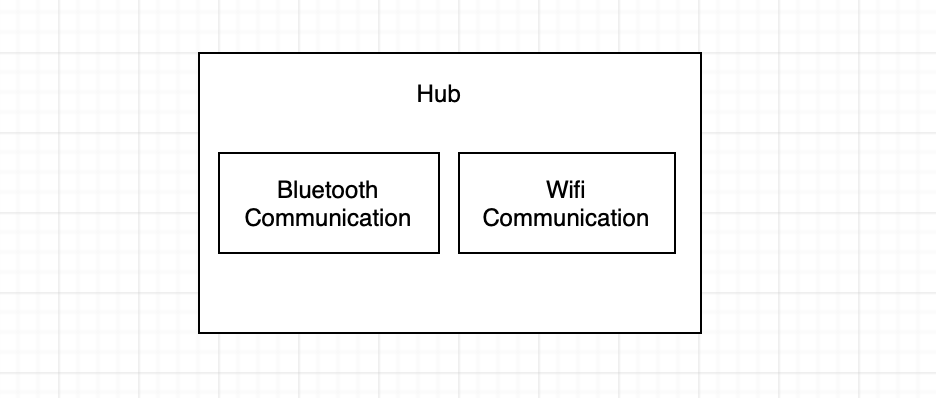
\includegraphics[width=0.60\textwidth]{images/Hub}
 \caption{Example subsystem description diagram}
\end{figure}

\subsection{WiFi Communications}
This is how the hub will take request from the mobile as well as sending data back to the mobile application

\subsubsection{Assumptions}
Users have an Android or iOS phone and users have not tampered with the hub and shutters.

\subsubsection{Responsibilities}
The hub should take request from the mobile application and send it acknowledgments for completed tasks.

\subsubsection{Subsystem Interfaces}
\begin {table}[H]
\caption {Subsystem interfaces} 
\begin{center}
    \begin{tabular}{ | p{1cm} | p{6cm} | p{3cm} | p{4cm} |}
    \hline
    ID & Description & Inputs & Outputs \\ \hline
    1 & Package all request and send to the hub & Subsystem 4.4 & Wifi Communication \\ \hline
    \end{tabular}
\end{center}
\end{table}

\subsection{Bluetooth Communications}
This is how the hub will take request from the mobile as well as sending data back to the mobile application

\subsubsection{Assumptions}
Users have an Android or iOS phone and users have not tampered with the hub and shutters.

\subsubsection{Responsibilities}
The hub should send request to designated shutters 

\subsubsection{Subsystem Interfaces}
\begin {table}[H]
\caption {Subsystem interfaces} 
\begin{center}
    \begin{tabular}{ | p{1cm} | p{7cm} | p{5cm} | p{3cm} |}
    \hline
    ID & Description & Inputs & Outputs \\ \hline
    1 &Package all request and send to the shutters& Bluetooth communication&Motor commands \\ \hline
    \end{tabular}
\end{center}
\end{table}